% Kompiuterijos katedros ir kibernetinio saugumo laboratorijos šablonas
% Template of Department of Computer Science II or cybersecurity laboratory
% Versija 1.3 2021 m. birželis [ March, 2015]

\documentclass[a4paper,12pt,fleqn]{article}
\usepackage[unicode,colorlinks=false]{hyperref}


\usepackage[utf8x]{inputenc}
%

\usepackage[L7x]{fontenc}
\usepackage{times}
\usepackage{ucs}
\usepackage{microtype}
\DisableLigatures{encoding = *, family = *}
 %package to switch the language
\usepackage{etoolbox}

  %set up of the page margins
\usepackage[top=2cm, bottom=2cm, left=3cm, right=1.5cm]{geometry}

 %1.1 line spacing
\linespread{1.1}


  %page numbering at the right side
\usepackage{fancyhdr}
\pagestyle{fancyplain}
\fancyhf{}
\renewcommand{\headrulewidth}{0pt} 
\fancyhfoffset[RO]{0cm}

  %to number at the bottom (exchange lines to number at the top)
\rfoot{\thepage}
  %\rhead{\thepage} %

% \usepackage[usenames,dvipsnames]{pstricks}
\urlstyle{same}
\hypersetup{
%  citecolor=Blue,
%  linkcolor=Blue,
%  urlcolor=Blue
pdfborder={0 0 0 }
}

 %for includegraphics
\usepackage{graphicx}



\usepackage[toc,page]{appendix}


\usepackage{caption}

 %for source codes
\usepackage{listings}
\lstset{commentstyle=\color{red},xleftmargin=10pt, framexleftmargin=6pt, numbersep=1mm, frame=single, numbers=left,numberstyle=\footnotesize,extendedchars=\true, inputencoding=utf8x,basicstyle=\footnotesize,extendedchars=true,
 keywordstyle=\color{black}\bfseries, breaklines=true, breakautoindent=true,framesep=8pt,linewidth=0.95\textwidth
}

 %for algorithms
\usepackage{algorithm}
\usepackage{algorithmic}
 %instead of the above two packages we can use algorithms2e
 %\usepackage[boxed,linesnumbered,vlined,slide]{algorithm2e}

 %special symbols
\usepackage{amsfonts}
\usepackage{amssymb}
\usepackage{amsmath}

 %for theorem like environments
\usepackage{amsthm}

 \usepackage{datetime}
 \renewcommand{\dateseparator}{--}


% SI system units
\usepackage{siunitx}
\sisetup{detect-all}
% Problem with fonts \SI{x.xx}{\micro\metre}, solved with updmap-sys --enable Map=utm.map
\renewcommand{\sfdefault}{uhv}
\renewcommand{\rmdefault}{utm}
\renewcommand{\ttdefault}{ucr}

% List management (itemize, etc.)
\usepackage{enumitem}

\newcommand*{\urlw}[1]{\href{#1}%
            {\nolinkurl{#1}}}

\numberwithin{equation}{section}


%%%%%%%%%%% lino įdėta
%
\usepackage{pifont,mdframed}

\newenvironment{warning}
  {\par\begin{mdframed}[linewidth=2pt,linecolor=red]%
    \begin{list}{}{\leftmargin=1cm
                   \labelwidth=\leftmargin}\item[\Large\ding{43}]}
  {\end{list}\end{mdframed}\par}
  

\usepackage{graphicx}
\graphicspath{{./images/}}

\newtoggle{inLithuanian}
 %If the report is in Lithuanian, it is set to true; otherwise, change to false
\settoggle{inLithuanian}{false}

%create file preface.tex for the preface text
%if preface is needed set to true
\newtoggle{needPreface}
\settoggle{needPreface}{false}

\newtoggle{signaturesOnTitlePage}
\settoggle{signaturesOnTitlePage}{false}


\theoremstyle{definition}
\newtheorem{definition}{\keyWordDefinition}
\newtheorem{example}{\keyWordExample}
\def\QED{\unskip\nobreak\hfill\kern5pt$\Box$}

\iftoggle{inLithuanian}{
%\usepackage[L7x]{fontenc}
\usepackage[english,lithuanian]{babel}

\newcommand{\todayiso}{\the\year \dateseparator \twodigit\month \dateseparator \twodigit\day}


\renewcommand{\today}{\number\year\space m. \space \ifcase\month\or
  sausio\or vasario\or kovo\or balandžio\or gegužės\or birželio\or
  liepos\or rugpjūčio\or rugsėjo\or spalio\or lapkričio\or
  gruodžio\fi
  \space\number\day\space d.}


 \usepackage{tocloft}
 \renewcommand\cftsecaftersnum{.} 
 \renewcommand\cftsubsecaftersnum{.} 
 \renewcommand\cftsubsubsecaftersnum{.}

 \usepackage{VUMIFKK}

 \DeclareCaptionLabelFormat{captionlt}{#2 #1}
   %smth is not fine with algorithms 
 \DeclareCaptionLabelFormat{captionltalg}{#2 #1 algoritmas}

 \usepackage{indentfirst}
 \renewcommand{\appendixtocname}{Priedai}
 \renewcommand{\appendixpagename}{Priedai}
 \renewcommand{\contentsname}{Turinys} 

 \renewcommand{\lstlistingname}{išeities kodas}
 \renewcommand{\figurename}{pav}
 \renewcommand{\tablename}{lentelė}


 \captionsetup*[lstlisting]{   
 labelsep=period,labelformat=captionlt
 }
 \captionsetup*[figure]{   
% labelsep=period,
 labelsep=space, %babel redefines pav to pav.
 labelformat=captionlt
 }
 \captionsetup*[table]{   
  labelsep=period,
  labelformat=captionlt
 }
 \renewcommand{\algorithmicrequire}{\textbf{Įvestis:}}
 \renewcommand{\algorithmicensure}{\textbf{Išvestis:}}

 \captionsetup*[algorithm]{   
 labelsep=period,labelformat=captionltalg
 }

\renewcommand{\thmhead}[3]{#2 #1#3}

}
{
%\usepackage[OT1,T1]{fontenc}
%\usepackage[L7x]{fontenc}



\usepackage[english]{babel}
\newcommand{\todayiso}{\twodigit\month \dateseparator \twodigit\day \dateseparator \the\year}
 \captionsetup*[algorithm]{   
 labelsep=period
 }
\captionsetup*[lstlisting]{   
 labelsep=period
 }
 \captionsetup*[figure]{   
 labelsep=period
 }
 \captionsetup*[table]{   
 labelsep=period
 }


}

%some kywords
 \def\keywordAbstract{\iftoggle{inLithuanian}{Santrauka}{Abstract}}
 \def\keywordAbstractOther{\iftoggle{inLithuanian}{Summary}{Santrauka}}
 \def\keyWordIntroduction{\iftoggle{inLithuanian}{Įvadas}{Introduction}}
 \def\keyWordConclusions{\iftoggle{inLithuanian}{Išvados ir rekomendacijos}{Conclusions and Recommendations}}

 \def\keyWordPreface{\iftoggle{inLithuanian}{Pratarmė}{Preface}}
 \def\keyWordAppendice{\iftoggle{inLithuanian}{Priedas}{Appendix}}
 \def\keyWordSignature{\iftoggle{inLithuanian}{parašas}{signature}}
 \def\keyWordDefinition{\iftoggle{inLithuanian}{apibrėžimas}{Definition}}
 \def\keyWordExample{\iftoggle{inLithuanian}{pavyzdys}{Example}}

\newcommand{\bothabstracts}[3]{
\setcounter{secnumdepth}{0}
\newpage
\hspace{2cm}
{\centering{\section{\keywordAbstract}}}

#1
\newpage
\hspace{2cm}
{\centering \section{\keywordAbstractOther}}

\begin{center}{\textbf{#2} }\end{center}

 #3
\setcounter{secnumdepth}{3}
}

 %non-numbered sections: #1 param: for labeling sec:#1, #2 -section title
\newcommand{\sectionWithoutNumber}[2]{\newpage
%\hspace{2cm}
\section*{#1}
\label{sec:#2}
\addcontentsline{toc}{section}{\nameref{sec:#2}}%{#3}
 }



\newcommand{\referenceSources}[1]{
\newpage
\cleardoublepage
\phantomsection
\iftoggle{inLithuanian}{
 \renewcommand{\refname}{Literatūros šaltiniai}

 \addcontentsline{toc}{section}{Literatūros šaltiniai}
 \markboth{\refname}{Literatūros šaltiniai}
 }
{

\addcontentsline{toc}{section}{References}
\markboth{References}{References}
}

\bibliographystyle{plain}
\bibliography{#1}
}



 \newcommand\authorsignature[1]{
\begin{flushright}
 \begin{minipage}[b]{0.45\textwidth}
  \centering
  \rule{\textwidth}{0.5pt}\\
   #1
  \end{minipage}
\end{flushright}
 }




 \newcommand\authorsignatures[5]{%
   \vspace{1cm}
   \authorsignature{#1}
   \ifstrequal{#2}{}{}{\vspace{0.3cm}
     \authorsignature{#2}
     \ifstrequal{#3}{}{}{\vspace{0.3cm}
      \authorsignature{#3}
      \ifstrequal{#4}{}{}{\vspace{0.3cm}
        \authorsignature{#4}
        \ifstrequal{#5}{}{}{\vspace{0.3cm}
         \authorsignature{#5}       
        }
      }
    }
} 
}

\newcommand{\authortitle}{
\iftoggle{signaturesOnTitlePage}{
\tiny{\keyWordSignature}
}{}
}

\newcommand{\depttitlepage}[8]
{
\thispagestyle{empty}
\begin{center}


\includegraphics[width=2cm]{jb_VU_zenklas}

%\vspace{-1cm}

\iftoggle{inLithuanian}
{ 
  VILNIAUS UNIVERSITETAS\\
  MATEMATIKOS IR INFORMATIKOS FAKULTETAS\\
  INFORMATIKOS INSTITUTAS\\
  <<KOMPIUTERINIO IR DUOMENŲ MODELIAVIMO KATEDRA>> ARBA \\ <<KIBERNETINIO SAUGUMO LABORATORIJA>>
}
{
  VILNIUS UNIVERSITY \\
  FACULTY OF MATHEMATICS AND INFORMATICS \\
  INSTITUTE OF COMPUTER SCIENCE\\
  DEPARTMENT OF COMPUTATIONAL AND DATA MODELING \\
}

\vspace{5cm}

#1\\
\vspace{0.5cm}
\textbf{\Large #2}
\end{center}

\vspace{5cm}


\hspace{0.5\textwidth}
\begin{minipage}{0.4\textwidth}
 \begin{flushleft} 
\iftoggle{inLithuanian}
{
 \ifstrequal{#3}{}{}{Atliko:\\[5pt]}
}
{
\ifstrequal{#3}{}{}{Done by:\\[5pt]}
}
%\noindent
\begin{tabular}{@{}lr}%\setlength\tabcolsep{0pt}
\ifstrequal{#3}{}{}{#3&\hspace{2cm}\authortitle\\[5pt]}
\ifstrequal{#4}{}{}{#4&\authortitle\\[5pt]}
\ifstrequal{#5}{}{}{#5&\authortitle\\[5pt]}
\ifstrequal{#6}{}{}{#6&\authortitle\\[5pt]}
\ifstrequal{#7}{}{}{#7&\authortitle\\}
\end{tabular}

\end{flushleft}

\end{minipage}

\vspace{0.5cm}
\hspace{0.5\textwidth}
\begin{minipage}{0.4\textwidth}
 \begin{flushleft} 

\ifstrequal{#8}{}{}
{

\iftoggle{inLithuanian}
{
Vadovas:
}
{
Supervisors:
}

#8

}

\end{flushleft}

\end{minipage}


\vfill

\begin{center}
Vilnius\\
\the\year
\end{center}

\iftoggle{needPreface}{
 \sectionWithoutNumber{\keyWordPreface}{preface}
Pratarmės (Preface) informacija


\iftoggle{inLithuanian}
{
\vspace{\baselineskip}\hfill
\today
}
{
 \vspace{\baselineskip}\hfill \today
}

 \vspace{5cm}

\iftoggle{signaturesOnTitlePage}{}
{
\authorsignatures{#3}{#4}{#5}{#6}{#7}
}
}{}
\newpage
}


\begin{document}
 % #1 -report type, #2 - title, #3-7 students, #8 - supervisor
 \depttitlepage{Information Technology II year}{Technical Specification\\{\small Software Engineering Project | Team 3}}{Titas Majauskas} 
 {Dinas Majauskas}{Jomantas Užusinas}{Vilius Juknevičius}{Sakalas Stasiulis}% students 2-5
 {Virgilijus Krinickij, Gediminas Rimša}

\tableofcontents


 %Introduction section: label is sec:intro
\newpage
\section{Purpose}

\subsection{Purpose of The Document}
The purpose of this document is to provide an overview of the whole system, while visualizing and explaining the main parts of a system via diagrams, technological decisions and verbal explanations. 

\section{Diagrams}

\subsection{System-context diagram}
\begin{center}
    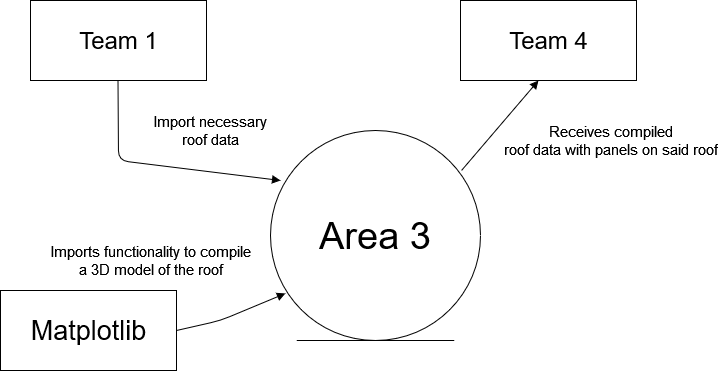
\includegraphics[scale=0.6]{main/images/system-context-diagram.drawio.png}
\end{center}
A \textbf{system context diagram}, shows \textbf{four} external objects that interact
with the solution's library. These objects have either arrows pointing to them or from them.\\ Arrow meaning:
\begin{itemize}
    \item An arrow line that points \textit{from the system to an object} - shows
what the \textbf{system provides} to that object.
    \item An arrow line that points \textit{from an object to the
system} - shows what that \textbf{object provides} to the system.
\end{itemize}
Objects meanings and purpose:
\begin{itemize}
    \item \textbf{Team 1} - will only act as a provider to the system. It will supply Area 3 with the necessary data about the roof, most likely in JSON format as primary format style.
    \item \textbf{Matplotlib} - will only act as a provider to the system. It will supply the whole solution with functionalities needed to compile a 3D model of the given roof and provide a visualisation of that model.
    \item \textbf{Team 4} - will act as a receiver of our library. Team 4 will receive the roof data that will be compiled through our algorithms. The format of the data sent to this team will be JSON as primary format.
\end{itemize}

\subsection{Activity diagram}
\begin{center}
    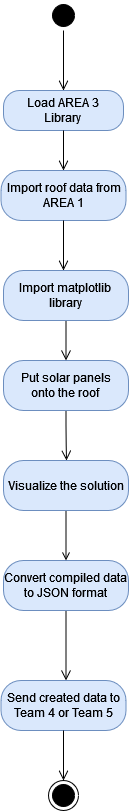
\includegraphics[scale=0.6]{main/images/Activity.drawio.png}
\end{center}
An \textbf{activity diagram} show the dynamic aspects of this solution. Our library provides \textbf{7} main activities, which work in coordination to provide our area's service.
To receive the end result, we have to complete these steps:
\begin{itemize}
    \item \textbf{Step 1} - having the library installed through \textit{PIP}, we will import the library to our system using the default python import module. Example: \textit{import solarPanelPlacer as spp}
    \item \textbf{Step 2} - after making our environment ready for data, we import the necessary roof data (roof polygons with their points), that will be extracted by Area 1. Primarily the data will be in JSON format and will be downloaded, imported into the working environment itself.
    \item \textbf{Step 3} - importing the \textbf{matplotlib} library, that we would have the necessary tools to the data that we are working with.
    \item \textbf{Step 4} - we run the algorithms, that will be imported through our library, to make optimized calculations on solar panel placement and place the panels on the roof. (the panels will be represented as polygons on said roof)
    \item \textbf{Step 5} - visualize our modified data using one of the \textbf{matplotlib} tools.
    \item \textbf{Step 6} - use our create function to convert our data into a JSON format.
    \item \textbf{Step 7} - send the formatted data to Team 4 and Team 5. The data transaction will be simplified as - our JSON file will appear in the working environment of the whole project, which will be accessible to the whole group from the launch of this system.
\end{itemize}

\subsection{Deployment diagram}
\begin{center}
    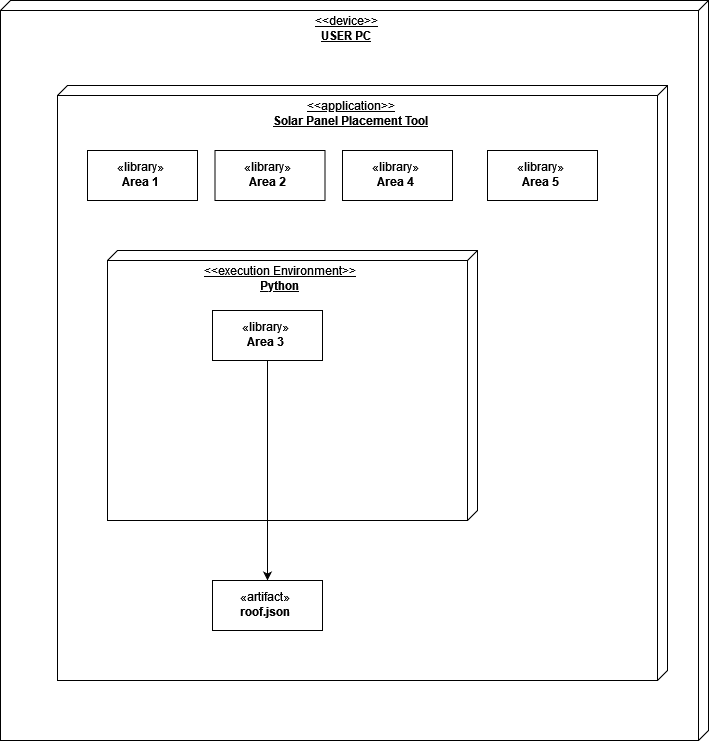
\includegraphics[scale=0.4]{main/images/deployment3.png}
\end{center}
\textbf{Deployment} diagram represents structural aspects of our area and how our solution will be working internally in the system. The main device is the \textbf{user's personal computer}. It will run our main application called \textbf{Solar Panel Placement Tool} - this application will consist of \textbf{five} libraries and will use only one execution environment - Python. Having in mind, that we are talking about our area, the only executable library at that moment will be \textbf{Area's 3} library. The library will be responsible for receiving the roof's data, making optimized calculations on said data and placing the solar panels onto the roof where it is possible, meaning that the solar panels will not be set onto chimneys, skylights and similar objects that are meaningfully put on the roof. After needed calculations, the data will be formatted back to JSON format and will be sent to another team.



\newpage
\section{Technological Decisions}
The library will be built using \textbf{Python} programming language in \textbf{Visual Studio Code IDE}. The library will be accessible to everyone through Python \textit{preferred installer program} (PIP). Its code will use \textbf{Git} version control, and all commits will be archived in a designated repository.\newline
For testing purposes our team will be using a Python testing framework called \textbf{Pytest}. 

\subsection{Visual Studio Code}
Visual Studio Code is a streamlined code editor with support for development operations like debugging, task running, and version control.

\subsection{Python}
Python is a programming language used for web and software development, data analytics, machine learning, and even design. Python will be used to implement required solution. We will use Python 3.11.0 - the newest version available (2022-10-25).

\subsection{Pytest/Pytest-Snapshot}


\begin{itemize}
    \item \textbf{Pytest} - a testing framework, which makes it easy to write small, readable tests, and can scale to support complex functional testing for applications and libraries.
    \item \textbf{Pytest-Snapshot} - a plugin for snaphshot testing with Pytest.
    Snapshot testing can be used to test that the value of an expression does not change unexpectedly.
\end{itemize}

\subsection{Python preferred installer program}
\textit{Python preferred installer program (PIP)} is used for installing libraries for Python.
\begin{itemize}
    \item \textbf{NumPy} - a Python library used for working with arrays. It also has functions for working in domain of linear algebra and matrices.
    \item \textbf{Matplotlib} - a comprehensive library for creating static, animated, and interactive visualizations in Python.
    \item \textbf{Mathutils} - a general math utilities library providing Matrix, Vector, Quaternion, Euler and Color classes.
\end{itemize}


\newpage
\section{Testing}
Given the testing framework our team will use, testing will be done on these said sections of our solution:
\begin{itemize}
    \item \textbf{Position:}
    \begin{itemize}
        \item Do testing to check if the position of the solar panel will not be crossed with position of chimneys, skylights, etc.
        \item Do testing to check if solar panels are not put over the roof's borders.
    \end{itemize}
    \item \textbf{Coverage}
    \begin{itemize}
        \item Do testing to check if solar panel covers the maximum possible area of the roof having in mind many limitations.
    \end{itemize}
\end{itemize}
For later, more complex testing \textbf{Pytest} plugin \textbf{Pytest-Snapshot} will be used to check if some changes happened while compiling the needed data.

\newpage
\section{Live version}
\begin{center}
    Overleaf read-only version - \href{https://www.overleaf.com/read/zkbzrtthrfcd}{\textit{click here}}\\
    Github repository for this documentation - \href{https://github.com/Jamtit/Technical-Requirements-Team3}{click here}
\end{center}

\end{document}